\documentclass[12pt, titlepage]{article}

\usepackage{booktabs}
\usepackage{tabularx}
\usepackage{hyperref}
\usepackage{listings}
\usepackage{graphicx}
\usepackage{caption}
\hypersetup{
    colorlinks,
    citecolor=black,
    filecolor=black,
    linkcolor=red,
    urlcolor=blue
}
\usepackage[round]{natbib}

%% Comments

\usepackage{color}

\newif\ifcomments\commentstrue %displays comments
%\newif\ifcomments\commentsfalse %so that comments do not display

\ifcomments
\newcommand{\authornote}[3]{\textcolor{#1}{[#3 ---#2]}}
\newcommand{\todo}[1]{\textcolor{red}{[TODO: #1]}}
\else
\newcommand{\authornote}[3]{}
\newcommand{\todo}[1]{}
\fi

\newcommand{\wss}[1]{\authornote{blue}{SS}{#1}} 
\newcommand{\plt}[1]{\authornote{magenta}{TPLT}{#1}} %For explanation of the template
\newcommand{\an}[1]{\authornote{cyan}{Author}{#1}}

%% Common Parts

\newcommand{\progname}{ProgName} % PUT YOUR PROGRAM NAME HERE
\newcommand{\authname}{Team \#, Team Name
\\ Student 1 name
\\ Student 2 name
\\ Student 3 name
\\ Student 4 name} % AUTHOR NAMES                  

\usepackage{hyperref}
    \hypersetup{colorlinks=true, linkcolor=blue, citecolor=blue, filecolor=blue,
                urlcolor=blue, unicode=false}
    \urlstyle{same}
                                


\begin{document}

\title{Verification and Validation Report: \progname} 
\author{\authname}
\date{\today}
	
\maketitle

\pagenumbering{roman}

\section{Revision History}

\begin{tabularx}{\textwidth}{p{3cm}p{2cm}X}
\toprule {\bf Date} & {\bf Version} & {\bf Notes}\\
\midrule
2024-04-15 & 1.0 & Initial Commit\\
\bottomrule
\end{tabularx}

~\newpage

\section{Symbols, Abbreviations and Acronyms}

\renewcommand{\arraystretch}{1.2}
\begin{tabular}{l l} 
  \toprule		
  \textbf{symbol} & \textbf{description}\\
  \midrule 
  CFD & Computational Fluid Dynamics\\
  DNS & Direct Numerical Simulation\\
  LES & Large Eddy Simulation\\
  MG  & Module Guide\\
  MIS & Module Interface Specification\\
  NFR & Nonfunctional Requirement\\
  SRS & Software Requirements Specification\\
  VnV & Verification and Validation\\
  \bottomrule
\end{tabular}\\

% \wss{symbols, abbreviations or acronyms -- you can reference the SRS tables if needed}

\newpage

\tableofcontents

\listoftables %if appropriate

\listoffigures %if appropriate

\newpage

\pagenumbering{arabic}

This document summarized the result of the verification and validation (VnV) process, as detailed in the \href{https://github.com/omltcat/turbulent-flow/blob/main/docs/VnVPlan/VnVPlan.pdf}{VnV Plan}. The requirements that were being tested are detailed in the \href{https://github.com/omltcat/turbulent-flow/blob/main/docs/SRS/SRS.pdf}{SRS}.

\section{Functional Requirements Evaluation}

\subsection{Verify Input [R1]} \label{ST:Input}
This requirement is covered by system test in section 4.1.1 of the VnV Plan. The test cases are designed to test the input validation and error handling. All test cases are passed. Test file: \href{https://github.com/omltcat/turbulent-flow/blob/main/test/system/test_system_input.py}{test\_system\_input.py} [VnV Plan 4.1.1]

\subsection{Generate Velocity Field [R2]} \label{ST:FieldGen}
This requirement is covered by system test in section 4.1.2 to 4.1.4 of the VnV Plan. The test cases are designed to test the calculation of meshgrid velocities in a field and test for the properties of the results. All test cases are passed. Test file: \href{https://github.com/omltcat/turbulent-flow/blob/main/test/system/test_system_eddy.py}{test\_system\_eddy.py}, \href{https://github.com/omltcat/turbulent-flow/blob/main/test/system/test_system_field.py}{test\_system\_field.py} [VnV Plan 4.1.2, 4.1.3, 4.1.4]

\subsection{Interface with CFD Software [R3]}
This requirement cannot be tested at current stage of development. This functionality is not implemented yet.

\section{Nonfunctional Requirements Evaluation}

\subsection{Accuracy [NFR1]}
This requirement cannot be tested at current stage of development. Providing realistic eddy profile is not implemented yet. [VnV Plan 4.2.1]

\subsection{Usability [NFR2]}
This requirement is not yet tested as it shares implementation with R3.

\subsection{Maintainability [NFR3]} 
The test for user to add a new shape function [VnV Plan 4.2.2] is not yet performed, but assuming it is, the result shall be presented as:

\begin{itemize}
  \item test subjects: x
  \item average time taken: x minutes
  \item percentage that still passed all tests: x\%
\end{itemize}

\subsection{Portability [NFR4]}

This requirement is tested by GitHub Actions running \progname{} on Linux, MacOS, and Windows runner. All tests are passed for the current version. Test results can be found on the \href{https://github.com/omltcat/turbulent-flow/actions/workflows/cross-platform.yaml}{GitHub Actions page}. [VnV Plan 4.2.3]
		
\subsection{Performance [NFR5]}
With inputs specified in Section 4.2.4 of the VnV Plan (10 million eddies in a $1000^3$ meshgrid), the program requires 24 GB of memory with estimated runtime of 50 minutes on an Intel i9-13900K processor. 

Discussions with Nikita Holyev about the expected use case revealed that the original requirement of ``minimal'' memory usage is not feasible, due to the shear size of the meshgrid in today's DNS/LES CFD simulations. 
	
% \section{Comparison to Existing Implementation}	

% This section will not be appropriate for every project.

\section{Unit Testing}
All unit tests covering every module developed for \progname{} are passed. The coverage report is shown in Figure \ref{fig:coverage}. The test results can be found on the \href{https://github.com/omltcat/turbulent-flow/actions/workflows/run-tests.yaml}{GitHub Actions page}.

\section{Changes Due to Testing}

% \wss{This section should highlight how feedback from the users and from 
% the supervisor (when one exists) shaped the final product.  In particular 
% the feedback from the Rev 0 demo to the supervisor (or to potential users) 
% should be highlighted.}

Other than bug fixes and minor improvements, the most significant change is direct result of performance testing and discussion with Nikita Holyev about potential real world use cases.

In the original MG and MIS design, each eddy is an abstract data type object created by the Eddy Module. The object stores eddy properties and methods to calculate velocities around it. This design is too slow for large scale use cases with many eddies (e.g. 10 million) and large meshgrid (e.g. $1000^3$). 

In the revised design, the Eddy Module is reduced to a library containing functions to calculate eddy velocity influences. The actual properties of all eddies are consolidated into the Flow Field Module as several arrays. This design allows NumPy to broadcast the calculation, greatly improving computing speed, with the trade-off of much increased memory usage.

To mitigate excessive memory usage and cut down unnecessary calculations between far away positions, a chunking approach is implemented to divide the entire meshgrid into smaller chunks, and calculate the velocity field for each chunk separately. 

The combination of these changes allows \progname{} to be usable in on regular personal computers with reasonable runtime and memory usage.

\section{Automated Testing} \label{sec:AutomatedTesting}

GitHub Action is used for Continuous Integration (CI). System and unit tests (made with pytest) are run whenever a pull request is made to the main branch. The command used for testing is as follows, which runs all test that are not designated as ``slow'' (those that take too long to finish), and checks if the coverage is above 95\%:

\texttt{ pytest --cov=src --cov-fail-under=95 -m "(unit or system) and not slow"}
		
\section{Trace to Requirements}
Please see Table \ref{Table:A_trace} for the traceability between system test cases and requirements. Note some tests are not yet performed.
\begin{table}[h!]
  \centering
  \begin{tabular}{|c|c|c|c|c|c|c|c|c|c|c|c|c|c|c|c|c|c|c|c|}
  \hline
                            & R1 & R2 & R3 & NFR1 & NFR2 & NFR3 & NFR4 & NFR5 \\
  \hline
  VnV Plan 4.1.1          & X  &    &    &      &      &      &      &      \\\hline
  VnV Plan 4.1.2          &    & X  &    &      &      &      &      &      \\\hline
  VnV Plan 4.1.3          &    & X  &    &      &      &      &      &      \\\hline
  VnV Plan 4.1.4          &    & X  &    &      &      &      &      &      \\\hline
  VnV Plan 4.1.5          &    &    & O  &      & O    &      &      &      \\\hline
  VnV Plan 4.2.1          &    &    &    & O    &      &      &      &      \\\hline
  VnV Plan 4.2.2          &    &    &    &      &      & O    &      &      \\\hline
  VnV Plan 4.2.3          &    &    &    &      &      &      & X    &      \\\hline
  VnV Plan 4.2.4          &    &    &    &      &      &      &      & X    \\\hline
  \end{tabular}
  \caption{Traceability Between Test Cases and Requirements, X indicated test passed and O indecates test designed but not yet performed}
  \label{Table:A_trace}
\end{table}
		
\section{Trace to Modules}

All unit test are passed, which covers all modules. Please see VnV Plan Section 5.2 for the traceability between test cases and modules.

\section{Code Coverage Metrics}

Coverage is tested with pytest-cov, using the command shown in Section \ref{sec:AutomatedTesting} that executes unit and system tests. An overall coverage of 98\% is achieved, with coverage report is shown in Figure \ref{fig:coverage}. 

\begin{figure}[h!]
\begin{center}
  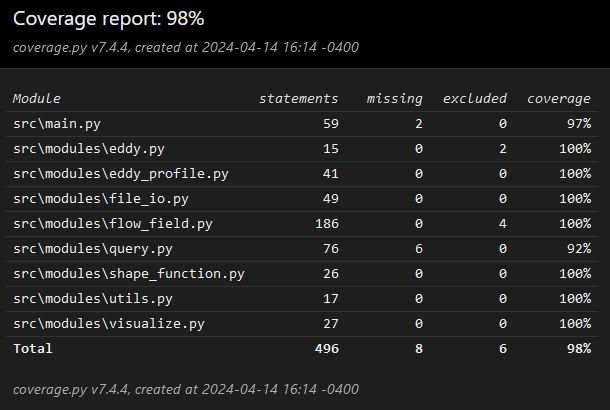
\includegraphics[width=0.8\textwidth]{img/coverage.png}
  \caption{Coverage report}
  \label{fig:coverage}
\end{center}
\end{figure}

The only two modules that are not fully covered are \texttt{main} and \texttt{query}. The not covered lines are either related to exception handling with those exceptions already tested in lower level modules, or impossible to reach in automated testing (e.g. plot pop-up).

% \bibliographystyle{plainnat}
% \bibliography{../../refs/References}

% \newpage{}
% \section*{Appendix --- Reflection}

% The information in this section will be used to evaluate the team members on the
% graduate attribute of Reflection.  Please answer the following question:

% \begin{enumerate}
%   \item In what ways was the Verification and Validation (VnV) Plan different
%   from the activities that were actually conducted for VnV?  If there were
%   differences, what changes required the modification in the plan?  Why did
%   these changes occur?  Would you be able to anticipate these changes in future
%   projects?  If there weren't any differences, how was your team able to clearly
%   predict a feasible amount of effort and the right tasks needed to build the
%   evidence that demonstrates the required quality?  (It is expected that most
%   teams will have had to deviate from their original VnV Plan.)
% \end{enumerate}

\end{document}